\section{Introduction}
{\addtocounter{table}{-3}} 

Icy moons, such as the Jovian moon Europa and the Saturnian moon Enceladus, likely feature large reservoirs of liquid water \cite{phillips2014europa}, \cite{thomas2016enceladus} and are of great scientific interest as potential hosts of simple alien lifeforms \cite{mckay2008possible}, \cite{chyba2001possible}, \cite{chyba2000energy}. A variety of mission concepts propose melting probes as the primary tool for the in-situ analysis of such cryosphere environments \cite{konstantinidis2015lander}, \cite{ulamec2006access}, \cite{dachwald2014icemole}.

A mathematical model for the propagation of a melting head through ice is well-established in the theory of \textit{Close-Contact Melting} (\gls{CCM}) \cite{moallemi1986analysis}, \cite{schuller2017spatially}. In this framework, a heat source pushed onto solid ice (e.g. by its gravitational force) induces a solid-liquid phase transition (Fig. \ref{subfig:ccmsketch}). The liquid phase is then modeled as an incompressible lubrication film. However, melting only occurs if the ambient pressure is sufficiently high.



\begin{figure}[ht!]
    \centering
    
    \begin{subfigure}[c]{0.49\textwidth}
    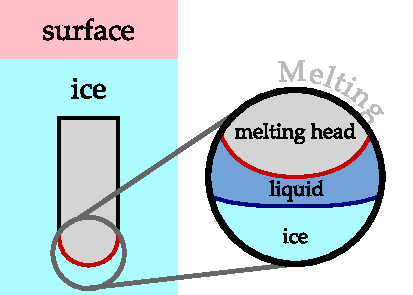
\includegraphics[trim={0cm 0.0cm 0.0cm 0.0cm},width=1\linewidth]{Chapters/Introduction/figs/probesIntroMeltingLiquid.pdf}
    \subcaption{Close-Contact Melting}
    \label{subfig:ccmsketch}
    \end{subfigure}
    \hfill
    \begin{subfigure}[c]{0.49\textwidth}
    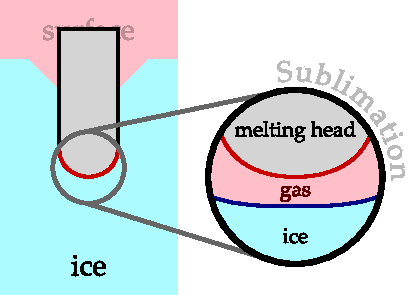
\includegraphics[trim={0.0cm 0.0cm 0.0cm 0.0cm},width=1\linewidth]{Chapters/Introduction/figs/probesIntroSublimation.pdf}
    \subcaption{Close-Contact Sublimation}
     \label{subfig:ccssketch}
    \end{subfigure}
    
    \caption[Melting Probes: Close-Contact Phase Change]{Concept sketch of close-contact phase change at the head of a melting probe moving through an icy environment. The liquid and gas film thickness is not shown to scale.}
    \label{fig:intro}
\end{figure}

In low-pressure environments, such as the near-vacuum conditions at the surface of many extraterrestrial bodies, solid-gas sublimation phase change is likely to occur (Fig. \ref{subfig:ccssketch}). This has severe implications for the design of melting probe trajectories, since the thermal and flow properties of gaseous lubricants differ significantly from those observed in a liquid melt film.

In this thesis, we extend the incompressible close-contact melting theory to compressible close-contact sublimation. We derive a model for non-isothermal gas lubrication with sublimation inflow, assuming a given ambient pressure and an ideal gas constitutive relation. We provide both the theoretical framework and the numerical implementation of a solver for equilibrium sublimation states, at which the interface propagation speed and sublimation film thickness are constant and a steady-state gas flow is assumed. We furthermore extent our model with slip boundary conditions derived from a macroscopic model for rarefied gas flows. The resulting new slip sublimation model predicts velocity and temperature discontinuities of first order in Knudsen and implements a first step towards a higher-order solver for close-contact sublimation in the rarefied regime.

The thesis is structured in five parts. In Chapter \ref{chap:review}, we will first introduce the most important concepts and review the theory our sublimation solver is based on. This includes a review of jump conditions across a phase-change interface and the theory of \textit{close-contact melting}. In this context, we briefly discuss an iterative solver for flux-driven melting proposed in \cite{schuller2019icarus}, which we extend to sublimation phase-change. We also review compressible lubrication theory, which serves as a model for the thin gaseous sublimation film. 
%The review includes model assumptions and simplified governing equations. 
Lastly, we introduce slip gas flows as a continuum limit of macroscopic models for rarefied gas flows. To obtain a close-contact sublimation model for the slip regime, we use boundary conditions recently introduced in \cite{beckmann2018evaporation} for the R13 equations.

In Chapter \ref{chap:compressible}, we propose a mathematical model for close-contact sublimation, based on compressible lubrication with an inflow boundary. Assuming a non-isothermal ideal gas lubrication film, we find a second-order differential equation of Reynolds type for the pressure distribution in the gas.
We discuss the influence of variations in Mach number, Reynolds number and temperature. We then proceed to use the model in a solver for the equilibrium sublimation state. In analogy to the close-contact melting solvers shown in \cite{schuller2017spatially}, \cite{schuller2019icarus} and \cite{schuller2016curvilinearccm}, we use an iterative strategy to find a film thickness that satisfies the conservation of energy across the phase-change interface (\textit{Stefan Condition}). 
To allow for a full coupling between pressure and temperature distributions in the gas, we introduce an additional nonlinear iteration.

In Chapter \ref{chap:nsfslipsolver}, we adapt the sublimation model to account for rarefaction effects at lower Knudsen numbers, using hydrodynamic slip boundary conditions derived in \cite{beckmann2018evaporation}. We then present a non-isothermal slip sublimation Reynolds equation, including the corresponding energy conservation and boundary conditions of first order accuracy in Knudsen.

Numerical results for two example single-species ($\textit{CO}_2$ and $\textit{H}_2\textit{O}$) sublimation scenarios at different ambient pressures are presented and discussed in Chapter \ref{chap:results}. 
We put particular emphasis on the equilibrium force-velocity curves, which link the contact force acting on the heater surface to a probe propagation speed for a given input power. These results are used to identify losses in sublimation efficiency, unique to compressible lubrication. Non-dimensional flow properties are shown for the different sublimation scenarios and model limits are assessed. We finally perform a parameter study of the slip sublimation model and show boundary velocity and temperature discontinuities for different Knudsen numbers.

All findings will be summarized in \chap{chap:conclusion} and, based on them, we will give suggestions for improvements and future work. 